\documentclass[tikz,border=4pt]{standalone}
% Shared art direction for the "phones" post, after Vagrancy's region art
% (vagrancy/analysis/art/regions.py and data/palette.json "art"): flat fills,
% plum ink lines, a mustard sky, peach and sage. Every colour below is copied
% from that palette so the post and the game look like one hand drew them.
%
% The scenes share a horizon at y=2.6 and the same sky band, so consecutive
% figures read as one continuous walk down the page.
\usetikzlibrary{arrows.meta,calc,decorations.pathmorphing}
\definecolor{ink}{HTML}{3B2A3F}
\definecolor{sky}{HTML}{E9C46A}
\definecolor{skylight}{HTML}{F2DC98}
\definecolor{cloud}{HTML}{F6E7B8}
\definecolor{peach}{HTML}{EBA77C}
\definecolor{peachdark}{HTML}{D98B5C}
\definecolor{cream}{HTML}{F3E6C4}
\definecolor{sage}{HTML}{9DB58A}
\definecolor{sagedark}{HTML}{6F8F66}
\definecolor{olive}{HTML}{B9B566}
\definecolor{teal}{HTML}{79ADA4}
\definecolor{tealdark}{HTML}{4F8580}
\definecolor{slate}{HTML}{6E8494}
\definecolor{stone}{HTML}{C9B79C}
\definecolor{wood}{HTML}{A9774E}
\definecolor{gold}{HTML}{E3B04B}
\definecolor{shadow}{HTML}{5B4A63}
\tikzset{
  ln/.style={draw=ink, line width=0.9pt, line join=round},
  thinln/.style={draw=ink, line width=0.6pt, line join=round},
  lab/.style={font=\sffamily\scriptsize, text=ink, align=center},
  tag/.style={font=\sffamily\scriptsize\bfseries, text=ink, align=center},
}
% A walking figure. #1 x, #2 y, #3 body colour, #4 head tilt in degrees
% (0 upright, negative looking down at a phone).
\newcommand{\walker}[4]{%
  \begin{scope}[shift={(#1,#2)}]
    \filldraw[fill=#3, ln] (-0.13,0) rectangle (0.13,0.52);
    \draw[ln] (-0.09,0) -- (-0.14,-0.28);
    \draw[ln] (0.09,0) -- (0.17,-0.26);
    \begin{scope}[rotate around={#4:(0,0.52)}]
      \filldraw[fill=cream, ln] (0,0.66) circle (0.14);
    \end{scope}
  \end{scope}}

\begin{document}
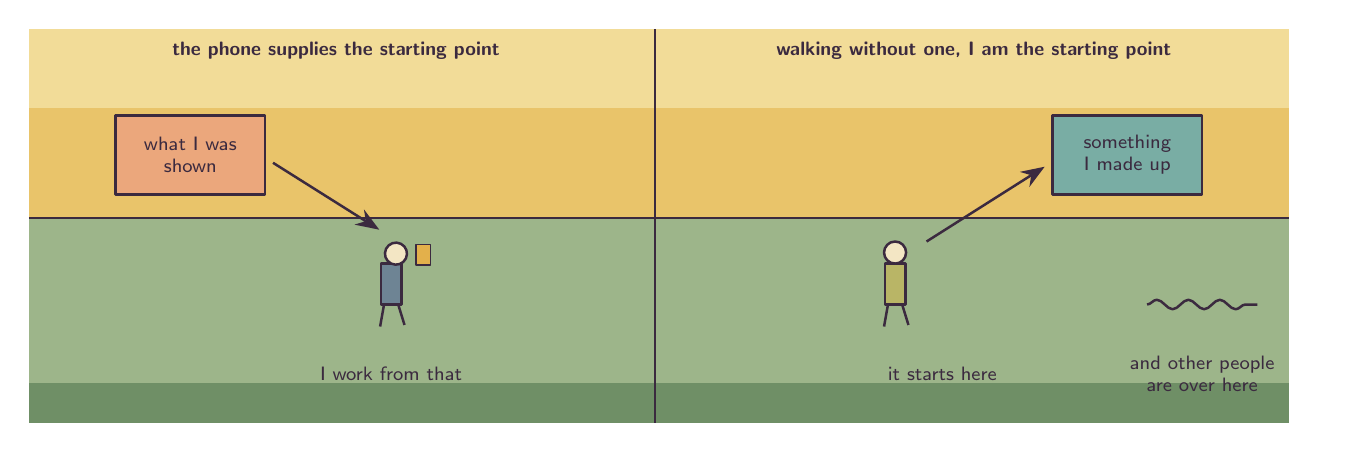
\begin{tikzpicture}[font=\sffamily]
  \fill[sky] (0,2.6) rectangle (16,5.0);
  \fill[skylight] (0,4.0) rectangle (16,5.0);
  \fill[sage] (0,0) rectangle (16,2.6);
  \fill[sagedark] (0,0) rectangle (16,0.5);
  \draw[ln] (0,2.6) -- (16,2.6);
  \draw[ln] (7.95,0) -- (7.95,5.0);
  % Left: the starting point is handed to the walker.
  \node[tag, text width=6.4cm] at (3.9,4.72) {the phone supplies the starting point};
  \walker{4.6}{1.5}{slate}{-26}
  \filldraw[fill=gold, thinln] (4.92,2.0) rectangle (5.1,2.26);
  \filldraw[fill=peach, ln] (1.1,2.9) rectangle (3.0,3.9);
  \node[lab, text width=1.7cm] at (2.05,3.4) {what I was\\shown};
  \draw[ln, -{Stealth[length=3mm]}] (3.1,3.3) -- (4.45,2.45);
  \node[lab, text width=2.6cm] at (4.6,0.62) {I work from that};
  % Right: the walker is the starting point.
  \node[tag, text width=6.4cm] at (12.0,4.72) {walking without one, I am the starting point};
  \walker{11.0}{1.5}{olive}{0}
  \filldraw[fill=teal, ln] (13.0,2.9) rectangle (14.9,3.9);
  \node[lab, text width=1.7cm] at (13.95,3.4) {something\\I made up};
  \draw[ln, -{Stealth[length=3mm]}] (11.4,2.3) -- (12.9,3.25);
  \node[lab, text width=3.2cm] at (11.6,0.62) {it starts here};
  % The caveat the post ends on, drawn rather than asserted.
  \draw[ln, decorate, decoration={snake, amplitude=0.6mm, segment length=4mm}] (14.2,1.5) -- (15.6,1.5);
  \node[lab, text width=3.1cm] at (14.9,0.62) {and other people\\are over here};
\end{tikzpicture}
\end{document}
